\documentclass[a4paper,12pt]{report}

\usepackage{alltt, fancyvrb, url}
\usepackage{graphicx}
\usepackage[utf8]{inputenc}
\usepackage{hyperref}
\usepackage{float}
\usepackage{textcmds}
\usepackage{a4wide}

\usepackage[italian]{babel}

\usepackage[italian]{cleveref}

\title{
\textbf{AirLine Traffic Simulator}
\\Relazione di progetto
\\Programmazione ad Oggetti
}
\date{Agosto 2021}

\author{
Severi Andrea
\\Foschi Andrea
\\Rodilosso Daniel
}

\begin{document}

\maketitle

\tableofcontents

% chapter 1
\chapter{Analisi}
Il gruppo si pone come obiettivo quello di realizzare un videogioco sulla gestione del traffico aereo, ispirandosi al gioco mobile \href{https://youtu.be/KTH084KeFBc}{\underline{“Flight Control”}}.
\\
L’obiettivo del giocatore sarà quello di far atterrare il maggior numero di aerei che compariranno progressivamente sulla mappa, evitando di farli collidere tra di loro (causando la fine del gioco).
\\
Il giocatore gestirà personalmente la direzione di ogni velivolo, disegnandone il percorso che dovrà seguire ciascun aereo, con il mouse.
\\
La difficoltà di gioco aumenterà con l’aumentare del numero di aerei che saranno fatti atterrare.

% 1.1
\section{Requisiti}
\paragraph{Funzionalità necessarie:}

\begin{itemize}
    \item Disegnare correttamente con il mouse il percorso che l’utente vuol far seguire al velivolo selezionato.
    
    \item Implementare un’intelligenza artificiale, che muoverà gli aerei quando non avranno una destinazione scelta dall’utente (l’aereo una volta entrato nella mappa non potrà uscire, ma dovrà continuare a volare all’interno di essa).
    
    \item Realizzare una gestione efficiente degli aerei in entrata sulla mappa e il relativo atterraggio quando raggiungeranno la pista di atterraggio.
    
    \item Salvataggio degli score dei vari utenti in un file apposito, che verrà reso disponibile ad ogni avvio.
    
    \item Gestione della difficoltà crescente durante la partita.
\end{itemize}

\paragraph{Funzionalità opzionali:}
\begin{itemize}
    \item Creazione e aggiunta di mappe dinamiche (es: implementazione di oggetti che causeranno la distruzione dell’aereo se sorvolati, animazioni dinamiche nella mappa).
    
    \item Implementazione suoni di gioco.
    
    \item Aerei speciali, con velocità diverse.
    
    \item Gestione del vento: questo causerà una maggiore o minore velocità degli aerei durante la partita.
\end{itemize}

\paragraph{\textbf{Challenge principali:}}
\begin{itemize}
    \item “Fluidità" delle animazioni (tracciamento della rotta, movimento degli aerei, atterraggio degli aerei, collisione tra gli aerei).
    
    \item Corretta implementazione del pattern MVC.
    \item Gestione della difficoltà (crescente durante la partita).
\end{itemize}

% 1.2
\section{Analisi e modello del dominio}
AirLine Traffic Simulator dovrà essere in grado di gestire lo spawn (Spawn) degli aerei (Plane) e la loro entrata in partita dopo un quantitativo di tempo prefissato. 
\\
È presente una \textbf{Mappa di gioco} (Seaside) a tema aeroporto.
\\	
All’inizio della \textbf{Partita} (Game) verranno creati e appariranno in maniera sequenziale gli \textbf{Aerei} sulla mappa, che seguiranno un \textbf{percorso casuale} (gli Aerei ancora non possiedono una rotta specifica da seguire ma semplicemente si muovono nella Mappa). 
\\
In questo caso quando un aereo non possiede una rotta specifica dovrà muovervi verso una direzione indicata dall’\textbf{algoritmo di I.A.}
\\
Compito dell’utente è quello di far atterrare gli Aerei sulle \textbf{Piste di Atterraggio} (AirStrip) presenti sulla mappa.
\\
Gli Aerei presenti nel gioco potranno essere di più tipologie (PlaneType), aventi velocità diverse.
\\
Un Aereo potrà atterrare quando sarà in prossimità dell’area di atterraggio, resa disponibile dalla Pista stessa.
\\
Sarà quest’ultima (AirStrip) a convalidare la possibilità o meno di fare atterrare il velivolo in caso di contatto con l'area di atterraggio.
\\
Per ogni Aereo che riuscirà ad atterrare correttamente, il Giocatore (User) incrementerà il proprio \textbf{Punteggio} con un valore deciso a priori.
\\
Il \textbf{Giocatore} potrà eseguire le seguenti operazioni sull’Aereo che vuole muovere:
\begin{itemize}
    \item selezionare l’Aereo che vuole controllare.
	\item disegnare il percorso (Path) che poi l'Aereo dovrà correttamente seguire.
\end{itemize}

\noindent È stato pensato di implementare degli indicatori all’interno dell'area di gioco per segnalare gli aerei in arrivo da fuori dalla Mappa.
\\
Questi segnali scompariranno non appena l’aereo entrerà in partita.

\paragraph{Il giocatore \underline{perde} se:}
\begin{itemize}
    \item fa collidere gli aerei tra di loro in volo
    \item urta il bordo con un aereo presente in partita
\end{itemize}
In entrambi in casi, viene generata un'esplosione a video.
\\
Nel tentativo di evitare ciò, allo scorrere del \textbf{Tempo di gioco}, altri aerei che dovranno essere fatti atterrare, compariranno sulla Mappa, con maggiore frequenza in base al punteggio.
\\
É possibile mettere anche in \textbf{pausa} la partita tramite pulsante dall’interfaccia di gioco.
\\
Alla fine della Partita, il Giocatore avrà ottenuto un punteggio finale, che sarà salvato su \textbf{file}. Se sarà sufficiente per entrare in \textbf{Classifica}, verrà inserito in quest’ultima.
\\
Dal \textbf{Menù Principale}, oltre che iniziare una nuova partita, si potrà visualizzare tale classifica.

% chapter 2
\chapter{Design}

% 2.1
\section{Architettura}
L’architettura di Airline Traffic Simulator segue l’architettura M.V.C. \newline
Abbiamo deciso di utilizzare il design classico di questo pattern.
\\
Utilizzando la libreria di JavaFX abbiamo un unione molto dipendente tra la parte di View e quella di Controller.
Questo perché la View stessa viene disegnata e implementata tramite un file .fxml, il cui scheletro deve essere presente all’interno del Controller.
Ciò genera da una parte un ottimizzazione per la realizzazione dei due componenti, dall’altra però va inevitabilmente a creare un forte legame di dipendenza.
In fatti nel caso in cui successivamente si volesse cambiare libreria grafica sostituendo JavaFx, la parte di Controller, andrebbe interamente riscritta, rendendo meno semplice la sostituzione in blocco della View stessa.
\\
AltSim implementa Seaside ed è il Controller centrale del sistema, ad esso sono infatti collegati i vari Controller degli oggetti chiave dell’applicazione (Plane, Map, Airstrip).
All’interno di Seaside l’utente sarà in grado di disegnare e controllare la rotta dei vari Plane che entreranno in partita.
Una particolare attenzione merita il GameEngine.
Esso si occuperà di monitorare i vari oggetti durante la partita (come ad esempio per il caso di Plane, verificare se collide con un altro Plane, o essendo in prossimità della AirStrip far atterrare il Plane stesso) e intraprendere le azioni di aggiornamento e notifica adeguati. Abbiamo riscontrato che un vantaggio di utilizzare questa architettura è che è possibile inserire altre Entità o modifiche all’interno del nostro gioco senza impattare la complessità di progettazione.
\begin{figure}[H]
    \begin{center}
        \centering
        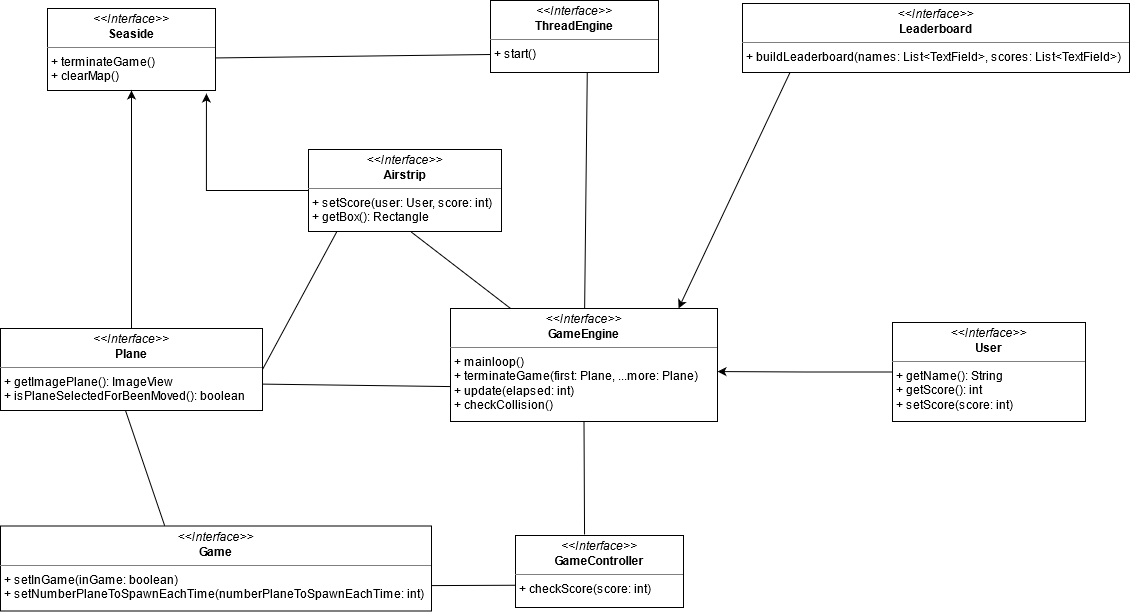
\includegraphics[width=\textwidth]{img/Design/Architettura.png}
    \end{center}
    \label{img:architettura}
\end{figure}

\clearpage

%2.2
\section{Design dettagliato}
\subsection{Severi Andrea}
Durante le fasi di analisi, è emersa l'esigenza di mantenere i dati relativi alle partite degli utenti in un file apposito e di estrapolarne una classifica contenente i migliori giocatori. Per cui, uno dei miei principali obiettivi era l'apportare un contributo per la creazione dell'utente e del salvataggio del suo punteggio.
\subsubsection{User}
Occupandomi personalmente dell'interfaccia grafica dell'applicazione, avevo subito in mente ogni singolo passo per la realizzazione dello \texttt{User}. 
Le sue caratteristiche sono l'univocità del nome utente da scegliere nel menù principale e il punteggio, attribuito successivamente in partita. Nonostante la scelta di soltanto due parametri, a mio vedere sufficienti per lo stato attuale dell'applicazione, ho deciso di utilizzare il pattern \textbf{Builder} per la creazione dell'utente. La motivazione è la predilezione per un pattern che fornisce chiarezza nella lettura del codice, rispetto a un costruttore, e per fornire una base solida di partenza nel caso di futura aggiunta di nuove caratteristiche da attribuire all'utente stesso.

\begin{figure}[H]
    \begin{center}
        \centering
        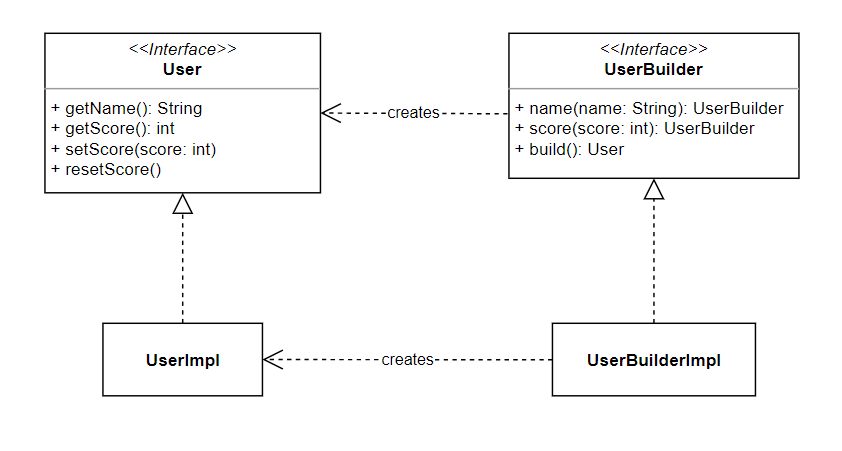
\includegraphics[width=\textwidth]{img/Design/Severi/User.png}
    \end{center}
    \caption{Creazione di \texttt{User}}
    \label{img:user}
\end{figure}

\subsubsection{UserRecords}
Al fine di mantenere in memoria la creazione degli utenti e dell'attribuzione loro di un punteggio, è stato necessario creare una classe che potesse gestire la realizzazione di una \textit{hidden directory} all' avvio dell'applicazione con al suo interno il file dei punteggi. Inizialmente, l'approccio scelto è stato la realizzazione della classe \texttt{RecordsValidation}, la quale controllava sia dell'esistenza di directory e file sia della creazione di essi. Tale metodo non era di mio gradimento, per cui ho deciso di separare le due parti di logica utilizzando il pattern \textbf{Adapter}, in modo tale da poter riutilizzare i metodi necessari anche per \texttt{UserRecordsImpl}, evitando ripetizioni di codice e violazioni del principio DRY. Per quanto riguarda l'interfaccia \texttt{UserRecords} ho optato per il pattern \textbf{Strategy}, in quanto contiene algoritmi utilizzabili per qualsiasi tipo di file si voglia usare. In prima battuta, la scelta è ricaduta su due estensioni: \textit{.csv} e \textit{.json}. La decisione di usare \textit{.json} è stata dettata dal fatto che è più facilmente manipolabile, grazie alla libreria \href{https://github.com/google/gson}{\underline{Gson}}, rispetto alla controparte, di cui è possibile trovare librerie di terze parti, ma che sono meno convincenti, data la scarsa accuratezza nell'attribuzione ai nomi dei metodi e il minor sviluppo da parte del team di creazione\footnote{In particolare si fa riferimento alla libreria \href{https://github.com/jtablesaw/tablesaw}{\underline{Tablesaw}}}. Per cui \texttt{UserRecordsImpl} contiene l'implementazione json degli algoritmi di inserimento, attribuzione del punteggio e controllo riguardo la presenza dell'utente nel file.
\begin{figure}[H]
    \begin{center}
        \centering
        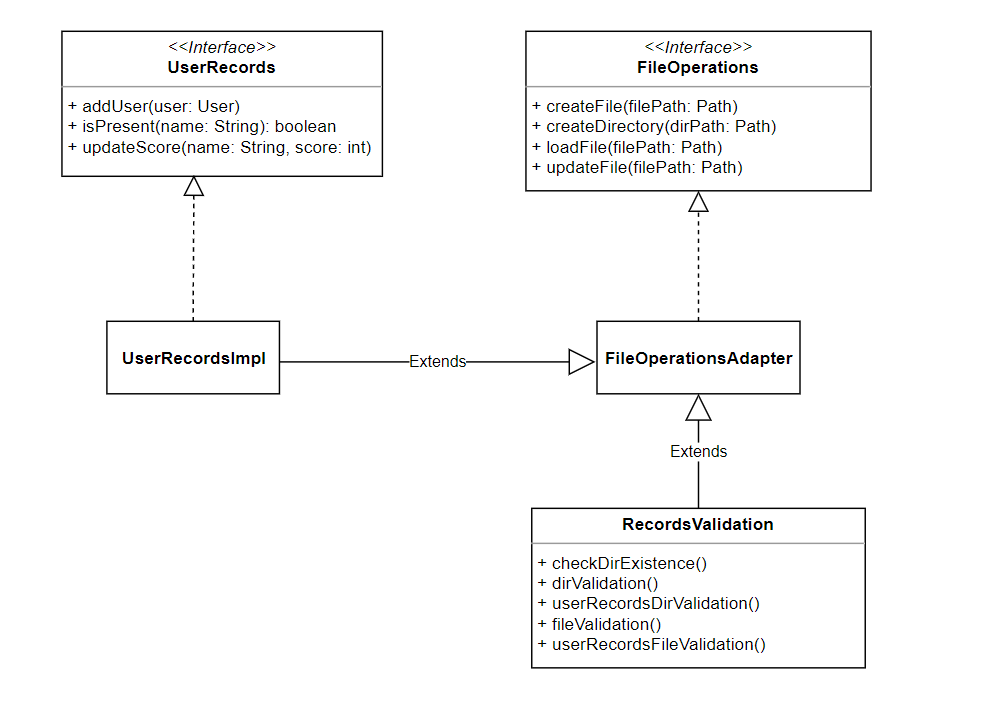
\includegraphics[width=\textwidth]{img/Design/Severi/Records.png}
    \end{center}
    \caption{Gestione del file}
    \label{img:records}
\end{figure}

\subsubsection{Leaderboard}
Per quanto riguarda la realizzazione della classifica ho pensato a un semplice algoritmo di comparazione fra gli utenti, basato ovviamente sul punteggio, volto all'utilizzo degli \textit{Stream}, introduzione nella versione 8 di Java, nonchè uno dei pilastri del corso. 
\begin{figure}[H]
    \begin{center}
        \centering
        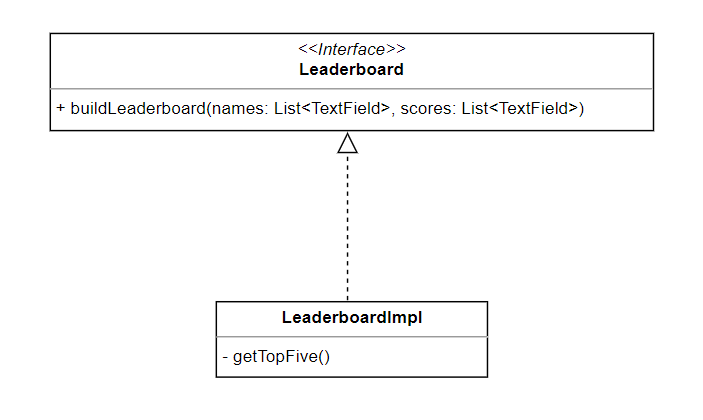
\includegraphics[width=\textwidth]{img/Design/Severi/Leaderboard.png}
    \end{center}
    \caption{Gestione della classifica}
    \label{img:leaderboard}
\end{figure}

\subsubsection{NameQuality}
La classe \texttt{NameQuality} consente di controllare il nome inserito dall'utente nel menù principale e di valutarne la qualità, facendo affidamento all'enum \texttt{NameResult}. Al fine di ottenere nomi semplici e di lunghezza finita, ho deciso di implementare un pattern regex, il quale restringe la scelta del nome a un lunghezza massima di 12 caratteri e l'utilizzo di soli numeri e lettere. In tal modo, l'input viene verificato tramite espressione regolare e viene ottenuto uno dei seguenti valori:
\begin{itemize}
    \item \qq{\texttt{CORRECT}}: il nome segue i canoni imposti
    \item \qq{\texttt{EMPTY}}: il nome è vuoto o contiene soli spazi
    \item \qq{\texttt{TOO\_LONG}}: il nome è più lungo di 12 caratteri
    \item \qq{\texttt{WRONG}}: il nome contiene caratteri non validi
    \item \qq{\texttt{TAKEN}}: il nome è già in uso
\end{itemize}
\noindent In base al valore ottenuto, successivamente si agisce in maniera diversa in interfaccia grafica. Tale scelta mi ha permesso di utilizzare spesso l'\texttt{Enum} nella View per inviare informazioni all'utente riguardo il nome selezionato.

\begin{figure}[H]
    \begin{center}
        \centering
        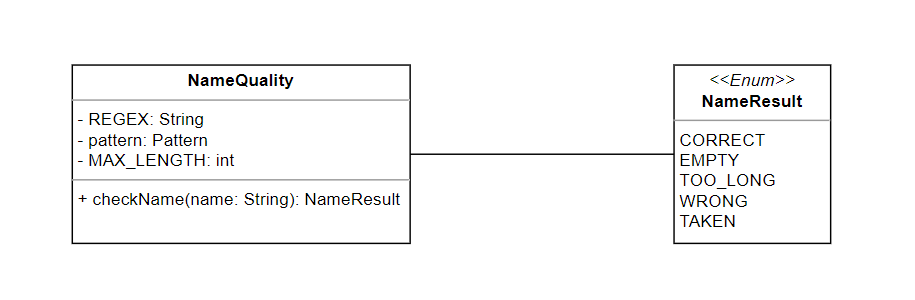
\includegraphics[width=\textwidth]{img/Design/Severi/Name.png}
    \end{center}
    \caption{Controllo sul nome}
    \label{img:name}
\end{figure}

\subsection{Foschi Andrea}
\subsubsection{Piste di atterraggio}
Mi sono personalmente occupato di una delle due componenti fondamentali del gioco: le piste di atterraggio. Tale componente si suddivide in due macrocategorie: quelle che gestiscono l’atterraggio degli aerei standard, e quelle che gestiscono l’atterraggio degli elicotteri (in realtà per quest’ultima categoria vi è nel codice una sola predisposizione a tale tipo di velivolo per implementazioni future, a causa della mancata implementazione degli elicotteri).
\begin{figure}[H]
    \begin{center}
        \centering
        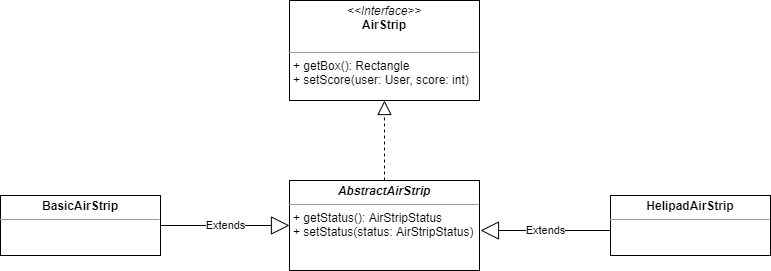
\includegraphics[width=\textwidth]{img/Design/Foschi/Airstrip.png}
    \end{center}
    \caption{Pista di atterraggio}
    \label{img:airstrip}
\end{figure}

\subsubsection{Atterraggio degli aerei e verifica delle collisioni}
Per fare in modo che la pista di atterraggio prenda in ingresso un aereo da far atterrare è stato necessario definire un controller del sistema. In questo modo la pista di atterraggio, tramite il metodo intersects() fornito da JavaFX, può accertare la collisione avvenuta e notificare l’evento alle altre componenti dell’applicazione. Si denota l’utilizzo dell’Enum AirStripStatus, che può assumere i seguenti valori:
\begin{itemize}
    \item \qq{\texttt{FREE}}: la pista è in grado di ricevere un aereo da far atterrare;
    \item \qq{\texttt{BUSY}}: la pista sta facendo atterrare un aereo e non è in grado di riceverne altri;
    \item \qq{\texttt{DISABLED}}: la pista è momentaneamente non disponibile.
\end{itemize}
\begin{figure}[H]
    \begin{center}
        \centering
        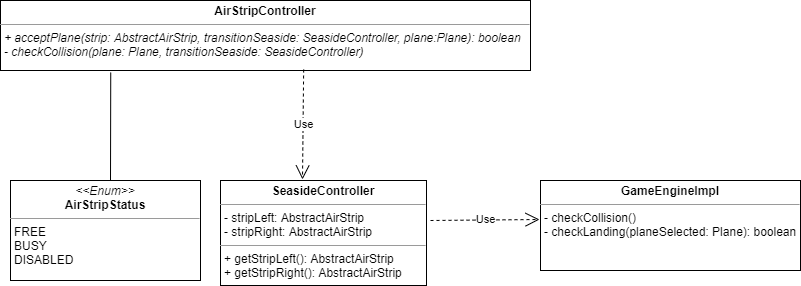
\includegraphics[width=\textwidth]{img/Design/Foschi/AirStripController.png}
    \end{center}
    \label{img:airstrip-controller}
\end{figure}

\clearpage

\subsection{Rodilosso Daniel}
\subsubsection{Plane}
Fin dall’inizio dello sviluppo del gioco si era d’accordo che l’entità Plane sarebbe stata un entità centrale nello sviluppo dell’applicazione.
La prima dinamica da affrontare è stato il movimento stesso del Plane:
\\
L’utente deve essere in grado di disegnare la propria rotta come più desidera e il Plane selezionato, essere in grado di seguirla.
\\
In una prima parte si è pensato far gestire lo scorrere delle coordinate campionate da Mouse, al GameEngineImpl che gestisce il gameloop
di gioco.
Prendendo una coppia di coordinate X e Y a tempo di frame, in questo modo si sarebbe vista un’animazione di movimento.
\\
Notando che l’ImageView della Sprite del Plane non seguiva però correttamente il percorso designato, si è deciso infine di utilizzare una 
libreria interna a JavaFx che risolveva efficacemente e con più precisione questo insorgere: la javafx.animation(in particolare la classe 
PathTransition).
\\
Le animazioni di movimento del Plane tutte e tre facenti parte della classe PathTransition hanno avuto il ruolo di occuparsi di:
	SpawnTransition: animazione eseguita durante lo spawn dei Plane in mappa
	RandomTransition: animazione causale del Plane quando è senza percorso.
	UserTransition: animazione disegnata dall’utente.
Una volta impostato il percorso del PathTransition, il Node (in questo caso l’ImageView del Plane che si deve muovere) e Orientation, questa 
è in grado di animare il nostro oggetto correttamente.
\\
Altra implementazione all’interno del Plane è stata creare una variabile per gestire il selezionamento del Plane su cui applicare i movimenti 
futuri.
Questo è stato reso possibile dopo aver implementato la variabile booleana isPlaneSelectedForBeenMoved.
Permettendo di capire quale Plane fosse stato precisamente selezionato, si poteva procedere ad eseguire le animazioni di quest’ultimo.
\\
Risolto l’obiettivo, si è pensato di creare diverse Sprite per rappresentare diversi tipi di Plane aventi anche velocità di gioco differenti.
Sprite possiede il metodo resizeSpriteToMap() per permettere di creare delle Sprite di grandezza in scala con la dimensione dello schermo 
utilizzato.
Le tipologie di Aerei differenti sono state raccolte all’interno del enum SpriteType mentre PlaneType permette di ottenere la velocità in 
base al tipo di Plane.
Questa funzionalità del differenziamento dei Plane però non è stata raggiunta rimanendo incompleta.
\begin{figure}[H]
    \begin{center}
        \centering
        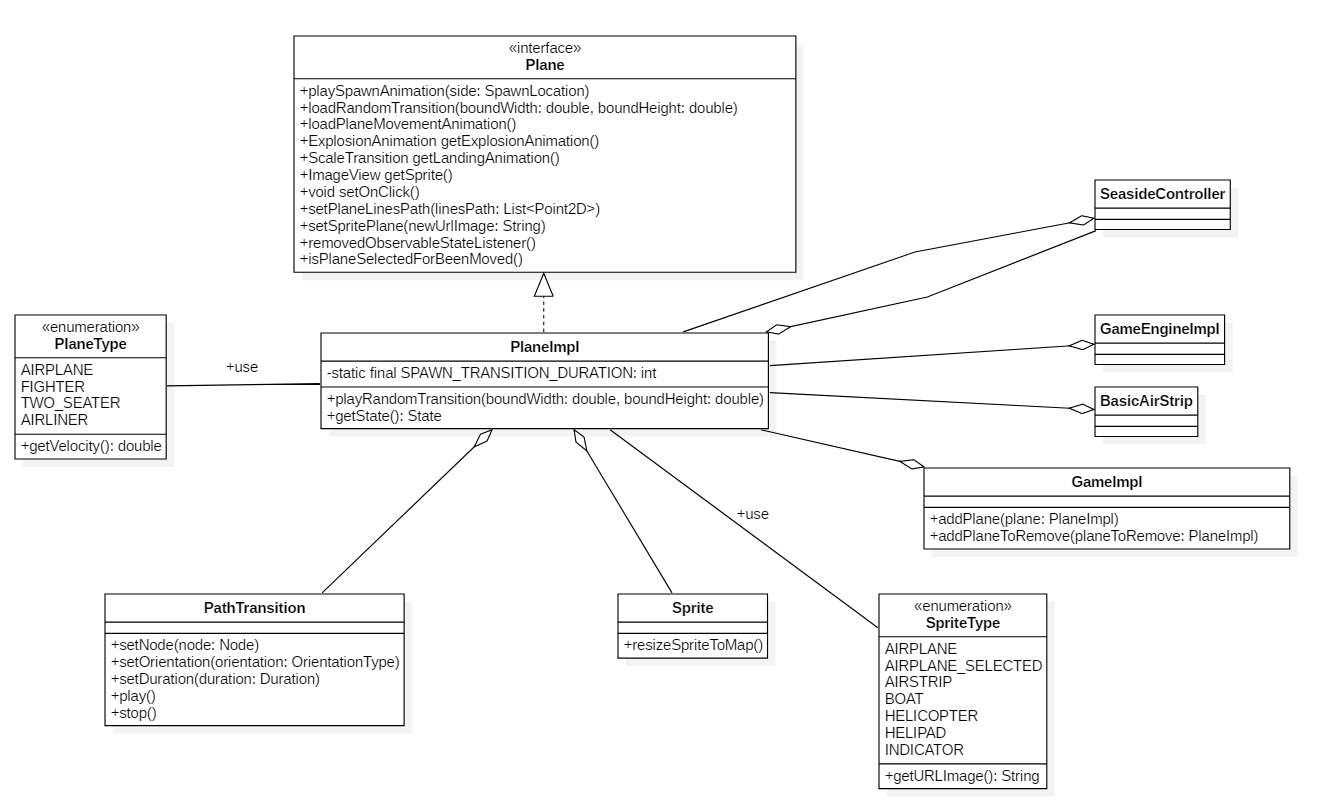
\includegraphics[width=\textwidth]{img/Design/Rodilosso/Plane.png}
    \end{center}
    \label{img:planeuml}
\end{figure}

\subsubsection{Seaside Controller}
La logica di View e Controller è racchiusa in questa classe, 
Possiamo considerarli due oggetti uniti tra di loro, la vista viene rappresentata da un file.fxml mentre il controller ne eredita lo 
scheletro di quest’ultimo quando viene lanciata l’applicazione.
\\
Compito di questa classe è far visualizzare la partita con tutti i suoi componenti e le animazioni che devono eseguire.
Riallacciandoci ai movimenti del Plane, tramite gli Event:
\begin{itemize}
    \item handlerMouseDragged()
    \item handlerMouseReleased()
\end{itemize}

\noindent Eseguiamo il campionamento delle coordinate tracciate dall’utente.
\\
Trasformiamo quest’ultime in oggetti della classe Point2D e le passiamo alle animazioni di movimento del Plane per eseguire lo spostamento a 
video.
\\
La classe Timeline permette invece di impostare un timer tramite il metodo setCycleCount(Animation.INDEFINITE);
Questo permette al SeasideController di avviare lo spawn continuativo dei Plane ogni tot. secondi.
\\
Tramite l’enumeration SpawnLocation viene assegnato una tra le quattro posizioni nella Mappa dove spawneranno i Plane e i loro indicatori di 
avviso.
\\
In parallelo al campionamento delle coordinate, avviene anche il disegno del percorso eseguito però ad opera della classe GraphicsContext,
sempre all’interno di SeasideController che si occuperà invece di ripulire la schermata stessa.
\begin{figure}[H]
    \begin{center}
        \centering
        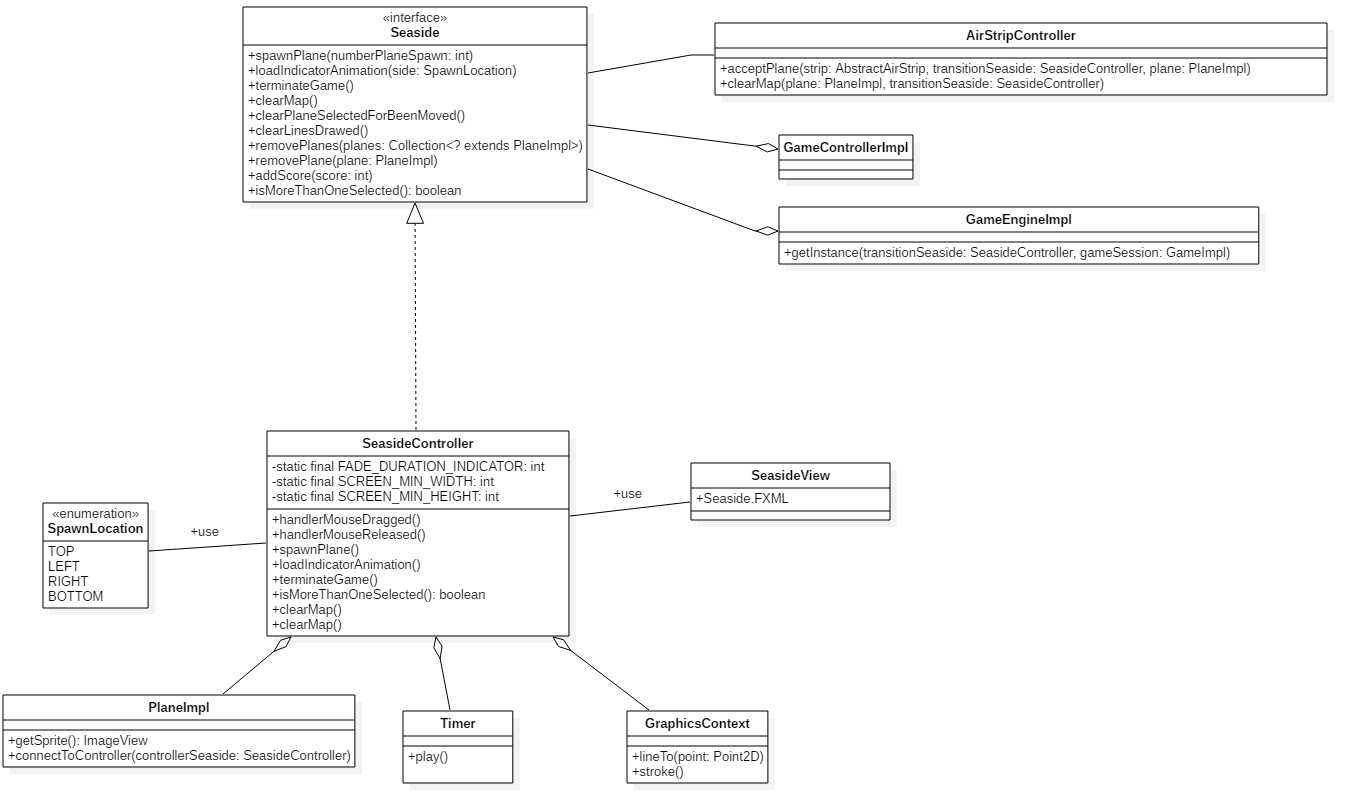
\includegraphics[width=\textwidth]{img/Design/Rodilosso/SeasideController.png}
    \end{center}
    \label{img:seaside-controller}
\end{figure}

\subsubsection{Animation}
Le animazioni vengono anch’esse visualizzate nella parte di View del SeasideController, questo perché necessitano del Thread principale 
JavaFx Application thread per essere eseguite.
\\
La superclasse Animation descrive generalmente le caratteristiche che saranno ereditate da ExplosionAnimation e LandingAnimation.
Il tutto ruota attorno alla ScaleTransition che è un animazione resa disponibile dalla libreria javafx e a un ImageView su cui applicare 
questo effetto.
\\
LandingAnimation essendo l’animazione di atterraggio del Plane, non fa altro che ereditare dalla superclasse senza inserire modifiche, 
mentre ExplosionAnimation che simula l’explosione, necessita di implementare un timer per lo scorrere delle immagini.
\begin{figure}[H]
    \begin{center}
        \centering
        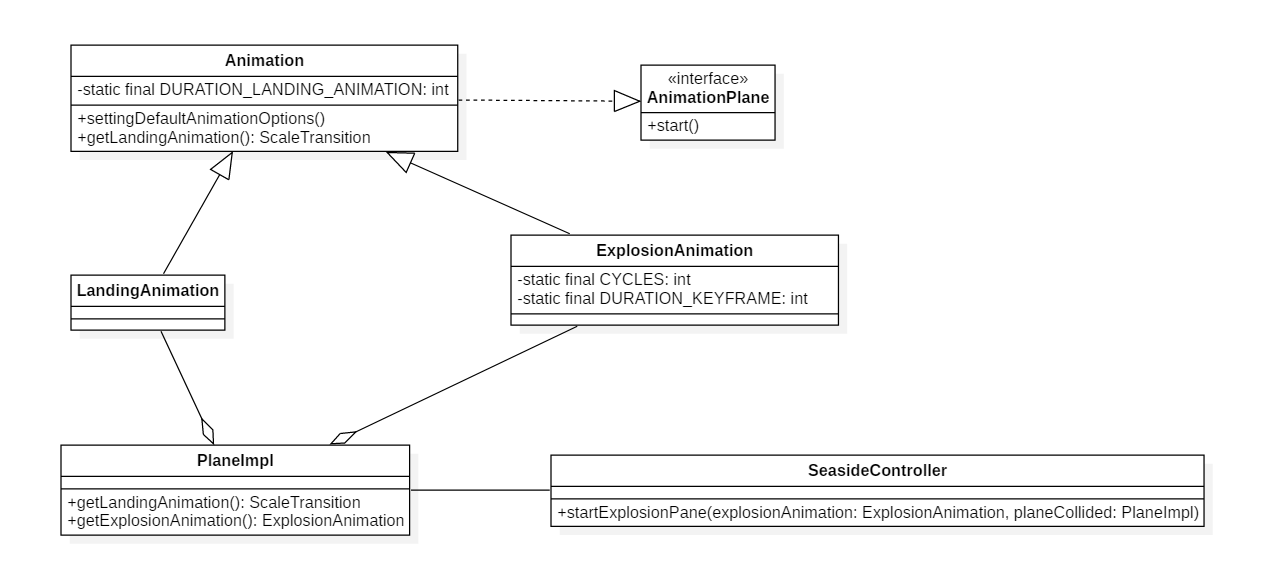
\includegraphics[width=\textwidth]{img/Design/Rodilosso/Explosion.png}
    \end{center}
    \label{img:explosion}
\end{figure}

\subsubsection{Game Loop}
Classe importante di controller è la classe GameEngineImpl.
Abbiamo deciso di utilizzarla come classe di monitoraggio per eseguire i vari controlli sui Plane in partita, essendo questi diversi.
Dialoga con SeasideController per eseguire alcune funzionalità sulla View.
L’istanza della classe viene lanciata dalla classe ThreadEngine, dovendo esserci un unico GameEngineImpl durante la partita ho deciso 
di applicare il pattern Singleton su di essa.
\\
Tramite il metodo principale mainLoop(), si avvia il ciclo di gioco, che ad ogni periodo, specificato sempre all’interno della classe, 
permette di eseguire le tre fasi di gioco importanti (init, update, render).
GameEngineImpl ogni periodo verifica:
\begin{itemize}
	\item se un Plane ha superato il bordo mappa, facendo esplodere il Plane e terminando la partita.
	\item Se un Plane è in zona atterraggio, eliminandolo e incrementando il punteggio a video.
	\item Se un Plane collide con un altro.
\end{itemize}

\noindent Questo controllo è stato reso possibile dalla funzione di libreria di javafx: intersects().
Grazie a questo metodo viene effettuato un controllo sulle dimensioni dei due Node monitorati e restituendo true o false se è avvenuta una 
collisione o meno.
Il GameEngineImpl gestisce anche i vari thread in partita eseguendo la terminazione di tutti con il metodo terminateGame() quando viene 
effettuata una collisione che termina la partita.
\\
Si è pensato a sviluppare un metodo che sostituisse intersects() e rendesse più riusabile questo controllo senza bloccarlo a un metodo di 
libreria, purtroppo però non si è riusciti nell’intento.
\begin{figure}[H]
    \begin{center}
        \centering
        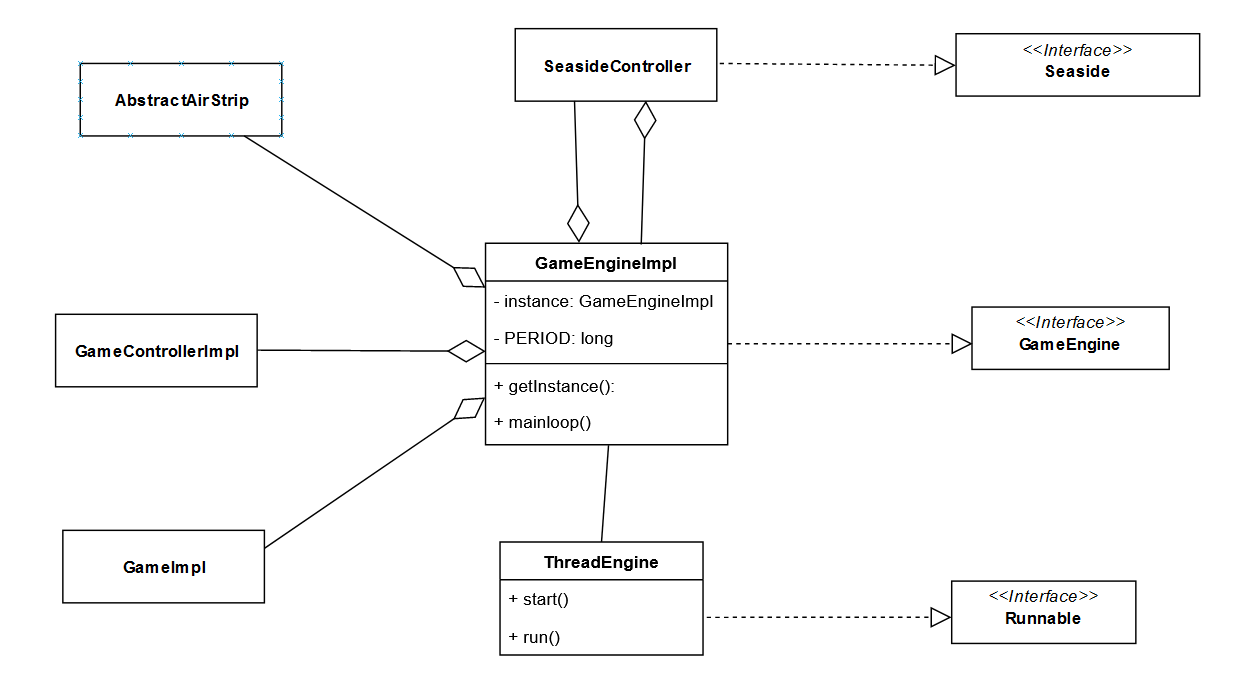
\includegraphics[width=\textwidth]{img/Design/Rodilosso/GameEngine.png}
    \end{center}
    \label{img:game-engine}
\end{figure}

\subsubsection{ObservableState}
Per gestire i vari stati del Plane durante la partita
mi sono fatto aiutare dalle Properties rese disponibili da Javafx che mi hanno permesso di realizzare questi controlli facilmente.
Inserendo questo ascoltatore sullo stato del Plane, mi ha permesso di modificare ed essere notificato ogni qualvolta avviene un cambio di 
stato permettendo di gestirlo in tempo ed eseguire le routine che sono collegate.
Nel caso del movimento casuale, questo deve attivarsi solamente quando il Plane è in stato di \qq{\texttt{WAITING}} da più di quattro secondi.
Senza un corretto ascoltatore come questo non sarebbe stato possibile avviare il timer al cambio di stato del Plane ed avviare successivamente 
lo spostamento casuale dell’Aereo.
\begin{figure}[H]
    \begin{center}
        \centering
        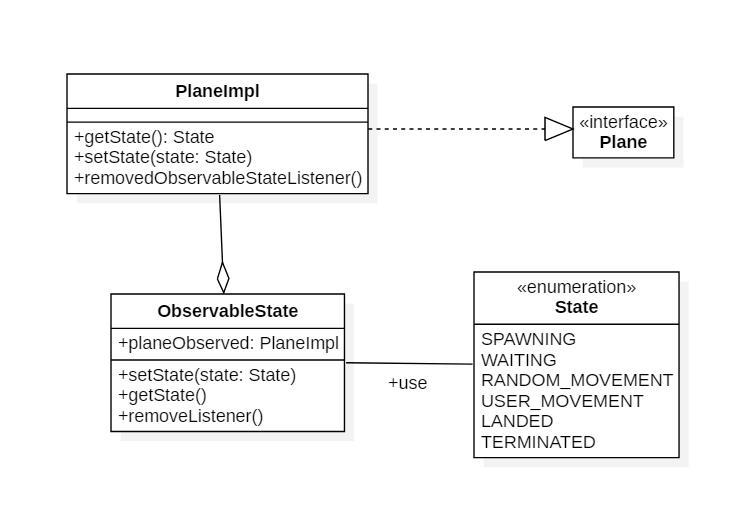
\includegraphics[width=\textwidth]{img/Design/Rodilosso/ObservableState.png}
    \end{center}
    \label{img:observable}
\end{figure}

% chapter 3
\chapter{Sviluppo}

% 3.1
\section{Testing automatizzato}
Per la realizzazione dei Test sull’applicativo abbiamo deciso fin da subito di utilizzare la libreria JUnit 5, inserendola nel build.gradle.
La logica di Test è stata scritta al fine di individuare possibili bug o imperfezioni durante lo sviluppo degli algoritmi più importanti.

\subsection{Severi Andrea}
Avendo sviluppato la parte di scrittura degli utenti su file, i test sono serviti sicuramente, affinchè si fosse pienamente sicuri che il tutto funzionasse correttamente. Difatti, inizialmente sono serviti per
verificare che la directory e il file venissero aggiornati in maniera appropriata, con la giusta indentazione e che la directory contenente il file fosse creata al primo avvio, anche nel caso in cui l'utente dovesse cancellare appositamente o erroneamente la directory stessa. Un'altra parte importante è stata controllare il nome dell'utente tramite espressione regolare. Non avendone mai sentito parlare prima, mi sono documentato prima di realizzare il regex che facesse al caso nostro. Infine la verifica della classifica è stata fondamentale, data l'importanza che ha all'interno dell'applicazione e il test ne ha verificato l'integrità.
\begin{itemize}
    \item LeaderboardTest
    \item UserRecordsTest
    \item NameQualityTest
\end{itemize}

\subsection{Foschi Andrea}
Per quanto riguarda la mia parte, ho deciso fosse opportuno effettuare alcuni test riguardanti il funzionamento delle piste di atterraggio, in particolare all’attribuzione del punteggio e all’interazione con gli user, oltre che alla gestione dello stato della pista. In tal modo, prima di poter implementare tali funzionalità nel codice, ho verificato che tutto funzionasse come mi sarei aspettato.
\begin{itemize}
    \item AirStripScoreTest
    \item AirStripStatusTest
\end{itemize}

\subsection{Rodilosso Daniel}
Dovendomi occupare anche della parte di View dell’applicazione mi sono venuti in aiuto alcuni Test sulle parti di logica scritte.
\begin{itemize}
	\item ExplosionAnimationTest
	\item GameEngineAreaTest
    \item PlaneImplTest
    \item SpriteTest
\end{itemize}

\noindent Un insidioso bug è stato risolto dopo aver eseguito un Test sulle coordinate.
In particolare la libreria di Animazioni di JavaFx PathTransition, quando vengono passati alla 
classe Path Point2D duplicati in successione, genera degli sfarfallii nel rendering delle ImageView, facendo sembrare come se l’immagine per un istante scomparisse dallo schermo, anche se invece è fisicamente presente.
In questo caso è stato sufficiente implementare il test removeDuplicateInLinesPathTest
di rimozione dei duplicati per risolvere il tutto.
\\
Altro bug degno di nota, è stato intercettato durante il Test manuale della View, nel movimento dei Plane.
Eseguendo il controllo del fuori bordo del Plane, ossia il verificare che il Plane non esca oltre le dimensioni della 
Mappa (SeasideController), ci si è accorti che quest’ultimo esplodeva senza motivo apparente.
La spiegazione del perchè erano i metodi della classe Node:
\begin{itemize}
    \item getBoundsInParent.getCenterX();
    \item getBoundsInParent.getCenterY();
\end{itemize}

\noindent In alcuni casi questi generano delle coordinate di errore negative, (nel nostro caso è stato riscontrato 
(-0.5, -0.5)) che essendo effettivamente fuori dalla Mappa di gioco, causavano l’esplosione inaspettate dei Plane, facendo terminare la partita.

% 3.2
\section{Metodologia di lavoro}
Abbiamo cercato fin da subito nella parte iniziale del progetto di suddividere in maniera equa il carico di lavoro da svolgere singolarmente.
Ci siamo soffermati sulla parte di Analisi lavorando insieme e confrontandoci sui possibili scenari e logiche da implementare per avere fin da subito una visione d’insieme dell’applicazione stessa.
Siamo riusciti quindi a creare la prima bozza di schema UML che abbiamo poi utilizzato durante tutto lo sviluppo per monitorare la realizzazione delle parti di ciascuno.
Nella fase iniziale abbiamo ritenuto necessario confrontarci diverse volte per poi proseguire in maniera parallela durante lo sviluppo.

\subsubsection{Version Control}
Abbiamo utilizzato Git come DVCS essendo quello più utilizzato.
Il branch principale è il “master”.
Quando si riteneva necessario sviluppare nuove funzionalità, veniva creato un branch “fix-*” dove tutti potevano inserire le proprie modifiche o nuove aggiunte senza intaccare il lavoro funzionante, per poi mergiare il tutto sul “master” dopo essersi trovati di comune accordo.
\subsection{Severi Andrea}
Realizzazione della parte grafica dell'applicazione tramite \texttt{JavaFX} con l'utilizzo di file fxml e css, e passaggio da una pagina all'altra tramite \textit{click} dei bottoni. 
\\
Realizzazione degli utenti e salvataggio su file degli stessi con creazione della cartella apposita. Costruzione della classifica sia livello grafico che logico. 
\\
Creazione dello spawn degli aerei e delle fasi di inizio, pausa e fine partita.

\subsection{Foschi Andrea}
Gestione delle piste di atterraggio e di tutti i suoi tipi (AirStrip, AbstractAirStrip, BasicAirStrip, HelipadAirStrip). Atterraggio degli aerei e notifica degli eventi. Verifica delle collisioni aereo-pista di atterraggio. Gestione generale della struttura MVC.

\subsection{Rodilosso Daniel}
Realizzazione dell’entità di gioco Plane e gestione dei movimenti di quest’ultima.
Disegno della rotta su schermo con successiva pulizia e campionamento dei punti da assegnare al Path del Plane.
Ideazione delle Animazioni sempre effettuate sui Plane in partita, in particolare di: ExplosionAnimation e LandingAnimation.
Ho continuato lo sviluppo della classe GameEngineImpl, assegnata al compagno Atanasov Atanas Todorov poi ritirato, realizzando successivamente i 
vari controlli di partita.
Ho partecipato alla realizzazione del controllo di collisione con il compagno Andrea Foschi.
Implementazione della classe Model di gioco GameImpl, per raccogliere le regole principali della logica applicativa.
Gestione della Mappa Seaside in parte, realizzazione grafica dei bouding box per l’atterraggio dei Plane.

% 3.3
\section{Note di sviluppo}
\subsection{Severi Andrea}
\begin{itemize}
    \item \textbf{JavaFX:} fondamentale la scrittura dei file fxml per ogni singola \qq{pagina} dell'applicazione, in quanto sono stati scritti quasi interamente a mano
    \item \textbf{Gson:} per la scrittura su file degli utenti (preferita a Jackson per preferenza personale per la chiarezza del codice)
    \item \textbf{Lambda:} fondamentale per una scrittura più minimale e comprensibile, usate spesso insieme a stream e programmazione funzionale
    \item \textbf{Programmazione funzionale e Stream:} utili per l'implementazione della classifica e della scrittura su file, nonchè per lo spawn degli aerei e la loro pausa durante la partita
    \item \textbf{Task:} per l'implementazione della barra di progresso all'avvio dell'applicazione
    \item \textbf{Gradle:} studio leggermente più approfondito per capire il codice Kotlin e per capire cosa facessero le parti fornite dai docenti
\end{itemize}

\subsection{Foschi Andrea}
\begin{itemize}
    \item Utilizzo di \textbf{JavaFX} che non è altro che il core principale della vista dell’applicazione.
    \item \textbf{Gradle:} mi sono personalmente occupato della gestione generale del progetto tramite Gradle, in modo che tutte le dipendenze con librerie esterne venissero rispettate. Mi è stato molto utile approfondire il suo funzionamento perché lo trovo uno strumento molto utile ed in grado di automatizzare una buona quantità di operazioni.
\end{itemize}

\subsection{Rodilosso Daniel}
\begin{itemize}
    \item \textbf{Lambda:} è risultato molto utile utilizzare le lambda expression perhè hanno reso il codice più pulito, leggibile e chiaro.
    \item \textbf{Stream:} utilizzati in alcuni casi particolari dove si sono rivelati molto utili, come per la rimozione delle coordinate duplicate e 
    per la rimozione degli oggetti Plane al termine della partita. Hanno permesso di alleggerire il codice delle funzioni.
    \item \textbf{JavaFX:}  il motore centrale dell’applicazione. Ha permesso la creazione di quest’ultima e alleggerito alcune sezioni altrimenti difficile da sviluppare da zero, come il caso della Animazioni di movimento, controllo collisioni, effetti grafici, gestione delle periferiche. Mi sono cimentato molto in questa libreria e mi ha appassionato molto la realizzazione di parti concrete e grafiche tramite una libreria grafica come questa.
\end{itemize}

% chapter 4
\chapter{Commenti finali}

% 4.1
\section{Autovalutazione e lavori futuri}
\subsection{Severi Andrea}
Questo progetto mi ha sicuramente aiutato a crescere come sviluppatore e mi ha fatto appassionare maggiormente a un linguaggio che inizialmente reputavo difficile e temibile, tanto dall'aver acquistato volumi quali \href{https://www.amazon.it/Effective-Java-Joshua-Bloch/dp/0134685997}{\qq{\underline{\textit{Effective Java}}}} e \href{https://it.wikipedia.org/wiki/Design_Patterns}{\qq{\underline{\textit{Design Patterns}}}}. Sono consapevole del fatto che ho ancora molto da migliorare, ma cerco sempre di documentarmi al meglio per trovare tecniche e approcci migliori alla scrittura del codice. Ho sempre cercato di rispettare regole (lingua inglese, stile) e convenzioni, affinchè il codice sia leggibile e comprensibile da tutti. Per il futuro voglio sicuramente concentrarmi su uno studio più approfondito dei Design Patterns e su una scrittura più professionale del codice, magari creando nuovi progetti da zero o andando a rimodellare quello appena creato. Inoltre conoscere sempre di più la programmazione ad oggetti che tanto mi ha appassionato, con lo studio possibilmente anche di altri linguaggi.

\subsection{Foschi Andrea}
Per me è stata la prima vera e propria esperienza in un progetto di grandi dimensioni, specialmente lavorando in gruppo dove la comunicazione è fondamentale. Sicuramente grazie a questa esperienza ho capito molto di più l’importanza di pensare nell’ottica di gruppo rispetto a quella del singolo. Complessivamente mi ritengo discretamente soddisfatto della parte da me svolta, nonostante sono consapevole di aver contribuito in maniera minore rispetto ai miei colleghi e spero che questo mi possa servire da lezione per impegnarmi di più in futuro.

\subsection{Rodilosso Daniel}
Sviluppare un videogioco in team è una cosa a cui ho sempre ambito, ringrazio per questo i professori, per la cura e precisione che 
hanno tenuto nella gestione di questo corso, permettendo appunto di poter realizzare dei progetti software da zero.
Ho accresciuto molto le mie conoscenze su Java e sul buon programmare in generale.
Queste conoscenze purtroppo le ho apprese nella parte finale del progetto.
In fatti mi rendo conto di alcune parti sviluppate con meno qualità rispetto ad altre.
Ammetto di non essere soddisfatto del mio operato quando vedo alcune parti gestite da me dove non ho applicato correttamente il pattern MVC o dove sono mancanti, questo assieme allo studio dei pattern in maniera più approfondita mi avrebbe permesso di portare il progetto ad una 
qualità maggiore. Ciò nonostante questo ha fatto crescere in me l’interesse per la parte di analisi in Java, ponendomi come sfida quello di approfondirli ancora 
di più e farne invece che di una parte occasionale, una costante.
Con la parte di View, la sua realizzazione e messa in funzione posso ammettere di essermi rimboccato le maniche e aver aiutato nella 
realizzazione in generale dell’applicazione, inserendo animazioni e logiche di gioco più carine. 
All’interno del gruppo mi sono trovato bene, nella prima fase di orientamento dovevo capire bene cosa fare e ammetto che questo mi ha fatto perdere delle settimane di produzione, però poi ho ingranato recuperando strada facendo. Il Team si è dimostrato sempre disponibile e collaborativo,
Abbiamo sempre discusso sulle parti di realizzazione e fix apertamente con mentalità rivolta al risolvere assieme tutti i problemi che sono comparsi. Mi dispiace infine per l’uscita finale del compagno Atanasov Atanas Todorov, che ha comunque, con le sue parti realizzate, collaborato e permesso la riuscita del progetto.

% 4.2
\section{Difficoltà incontrate e commenti per i docenti}
\subsection{Severi Andrea}
Come gruppo, nonostante la comunicazione costante, è sicuramente mancata un po' di sintonia, conoscendosi poco e sarebbe servita una migliore organizzazione, in modo tale da non riscrivere parti già fatte e concentrarsi maggiormente sui propri punti. Forse poteva servire per evitare di fallire la deadline precedente. 
Il corso mi ha aiutato a ragionare molto di più sul problema da risolvere, piuttosto che buttarsi subito sulla scrittura di codice. Nonostante sia un corso difficile, ho apportato il massimo impegno e penso ciò verrà ripagato.
Una cosa che non mi è piaciuta a pieno è stata la spiegazione su JavaFX, poichè non ero bene a conoscenza di ciò che realmente offre e che pensavo si dovesse implementare da zero. Nonostante questo, corso fatto molto bene.

\subsection{Foschi Andrea}
All’interno del gruppo si è respirato sicuramente un clima collaborativo. Tuttavia, a mio parere è un po’ mancata l’organizzazione, tanto che abbiamo fallito una deadline, oltre al fatto che un collega ha dovuto abbandonare il progetto proprio quando eravamo alla fine per cause di forza maggiore. Personalmente ho trovato il corso più complicato finora, ma anche quello più interessante. Avrei preferito avere più indicazioni in merito allo sviluppo del progetto in sé, ad esempio approfondendo più sul Game Programming o sull’uso di librerie esterne, ma mi rendo anche conto che il numero di ore è limitato. Personalmente come piccola modifica chiederei di alleggerire una delle due valutazioni per il voto finale (progetto o prova pratica), perché per come ho vissuto il corso mi sembra più pesante di altri da 12 CFU.
            
\subsection{Rodilosso Daniel}
Il corso di Programmazione ad Oggetti è un corso veramente di alta qualità.
In una prima parte non ne sono stato colpito, ma poi con l’arrivo del progetto da sviluppare e la messa in atto di ciò, mi sono appassionato sempre di più a questo mondo.
Mondo approfondito in maniera sempre accurata e precisa dai professori, che permettono una volta terminato, di avere delle solide basi nel mondo della programmazione e del clean-code, indispensabile per realizzare applicazioni di qualsiasi genere.

\appendix
\chapter{Guida utente}
\section*{Home Page}
All'avvio dell'applicazione, sono presenti 4 pulsanti: \texttt{START, LEADERBOARD, CREDITS, EXIT}, rispettivamente per avviare una nuova partita, visualizzare la classifica dei migliori giocatori, visionare i riconoscimenti per ognuno dei membri del gruppo e uscire dall'applicazione.
\begin{figure}[H]
    \begin{center}
        \centering
        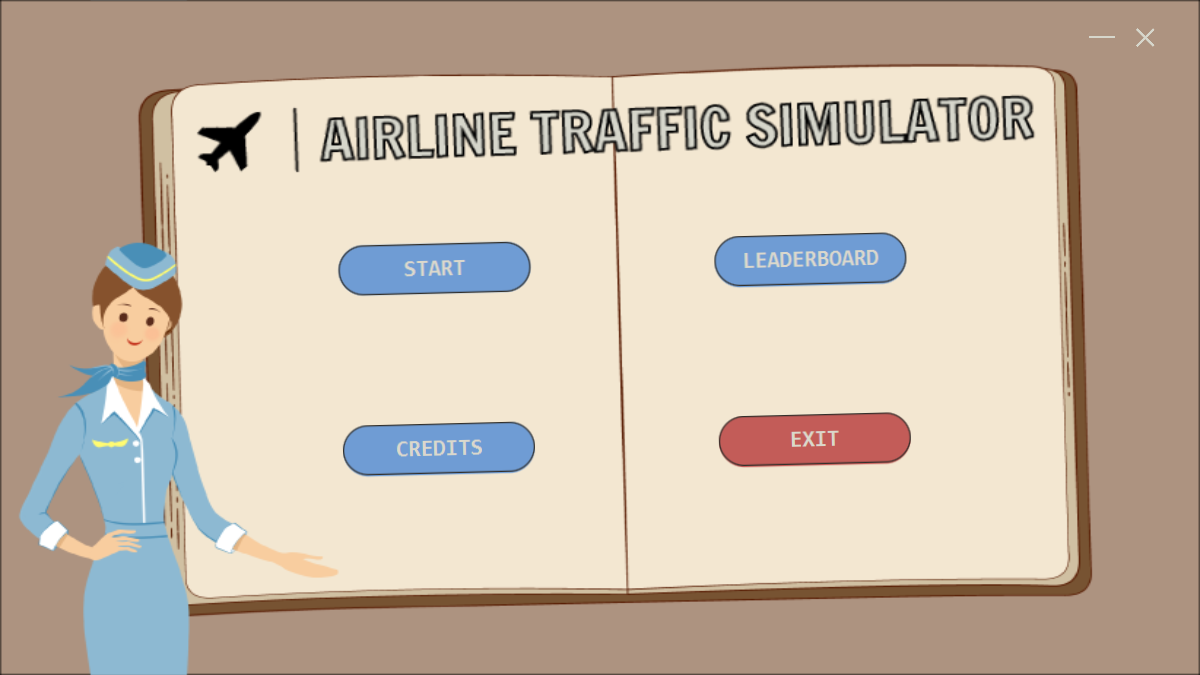
\includegraphics[width=\textwidth]{img/GuidaUtente/Home.png}
    \end{center}
    \caption{Home Page}
    \label{img:homepage}
\end{figure}

\section*{MapChoice}
Tramite questa schermata è possibile scegliere una delle mappe disponibili, al momento solo una delle quattro. Inoltre è obbligatorio scegliere un nome, come suggerisce l'info per iniziare una nuova partita.
\begin{figure}[H]
    \begin{center}
        \centering
        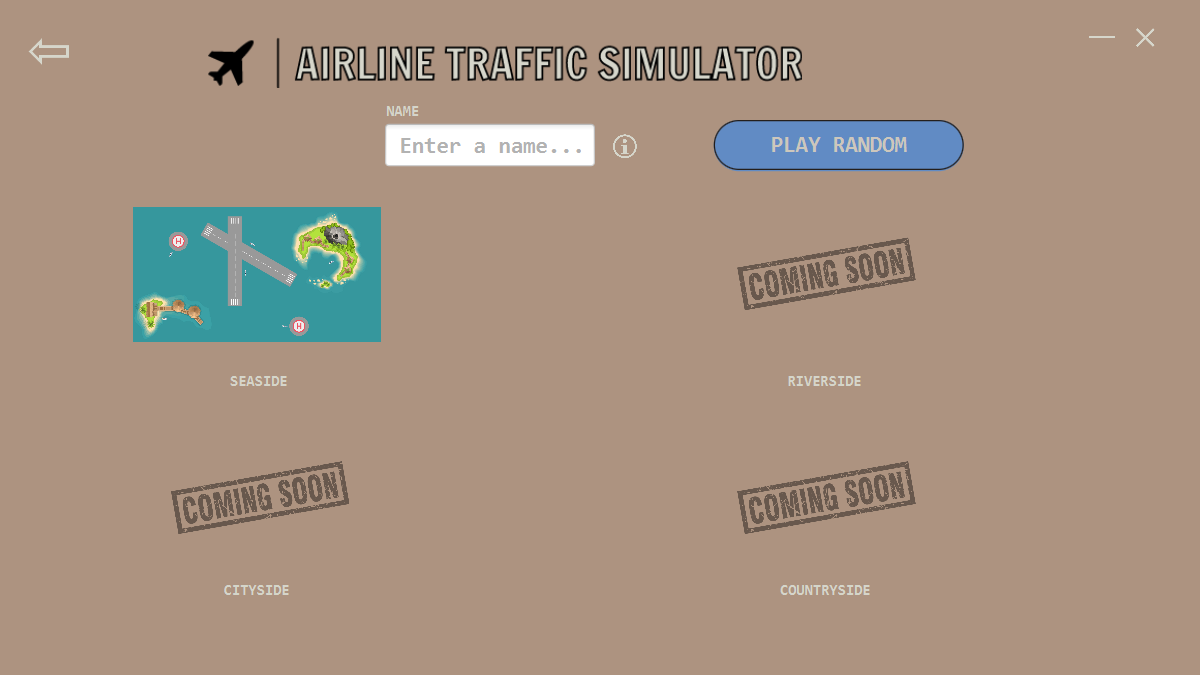
\includegraphics[width=\textwidth]{img/GuidaUtente/MapChoice.png}
    \end{center}
    \caption{Scelta della mappa}
    \label{img:mapchoice}
\end{figure}

\clearpage

\section*{Classifica}
In questa schermata è possibile vedere la top 5 (inizialmente vuota) dei migliori giocatori di AirLine Traffic Simulator con relativo nome e punteggio.
\begin{figure}[H]
    \begin{center}
        \centering
        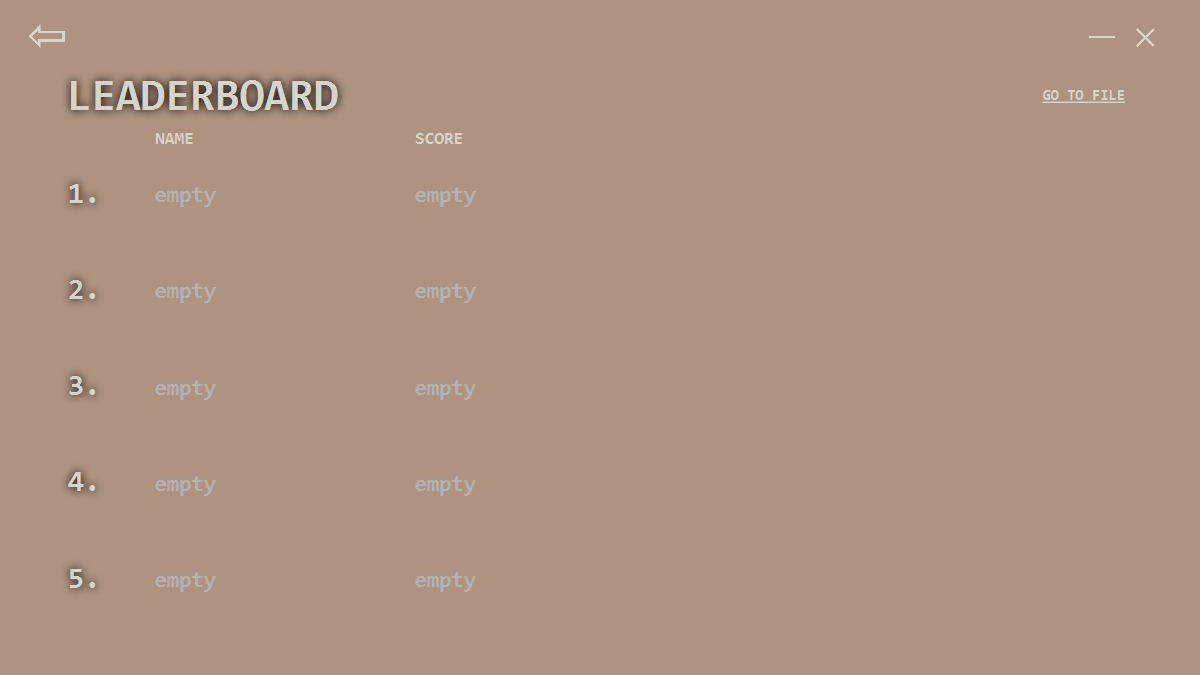
\includegraphics[width=\textwidth]{img/GuidaUtente/Leaderboard.png}
    \end{center}
    \caption{Classifica}
    \label{img:leaderboard-png}
\end{figure}

\clearpage

\section*{Credits}
Schermata per una veloce visione del lavoro svolto dai singoli partecipanti al gruppo.
\begin{figure}[H]
    \begin{center}
        \centering
        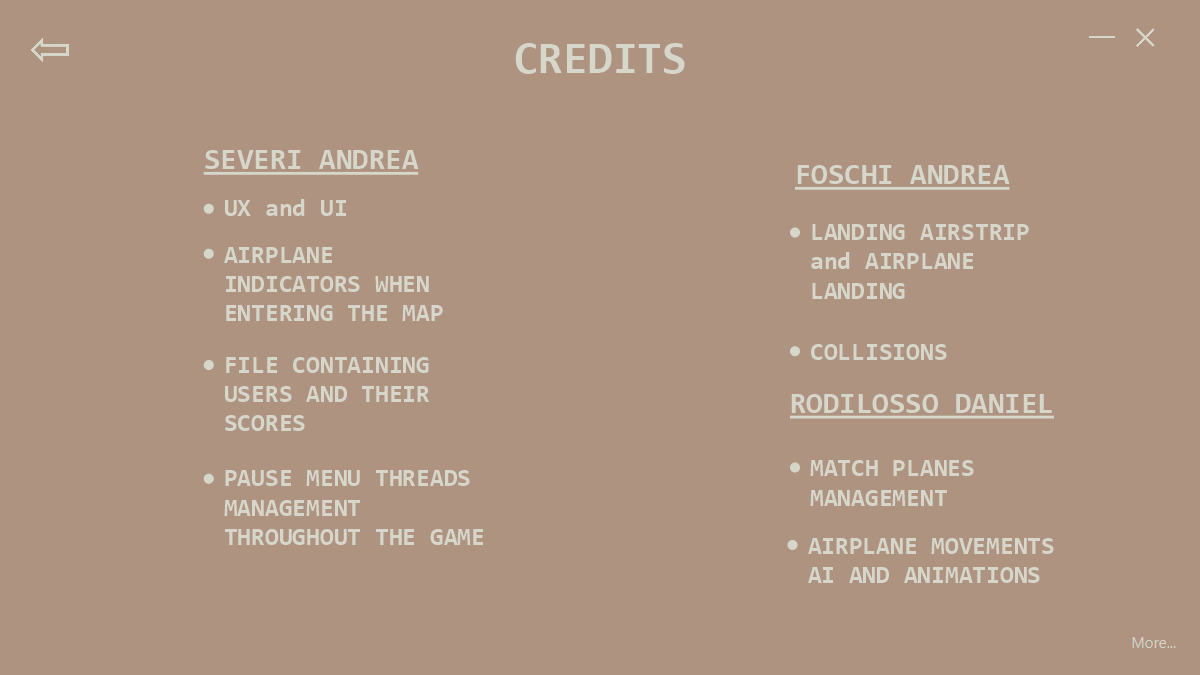
\includegraphics[width=\textwidth]{img/GuidaUtente/Credits.png}
    \end{center}
    \caption{Riconoscimenti}
    \label{img:credits}
\end{figure}

\clearpage

\section*{Partita}
All'avvio della partita, la mappa Seaside si presenterà così con l'opzione di poter mettere in pausa il gioco e uscire o riprendere successivamente.
\begin{figure}[H]
    \begin{center}
        \centering
        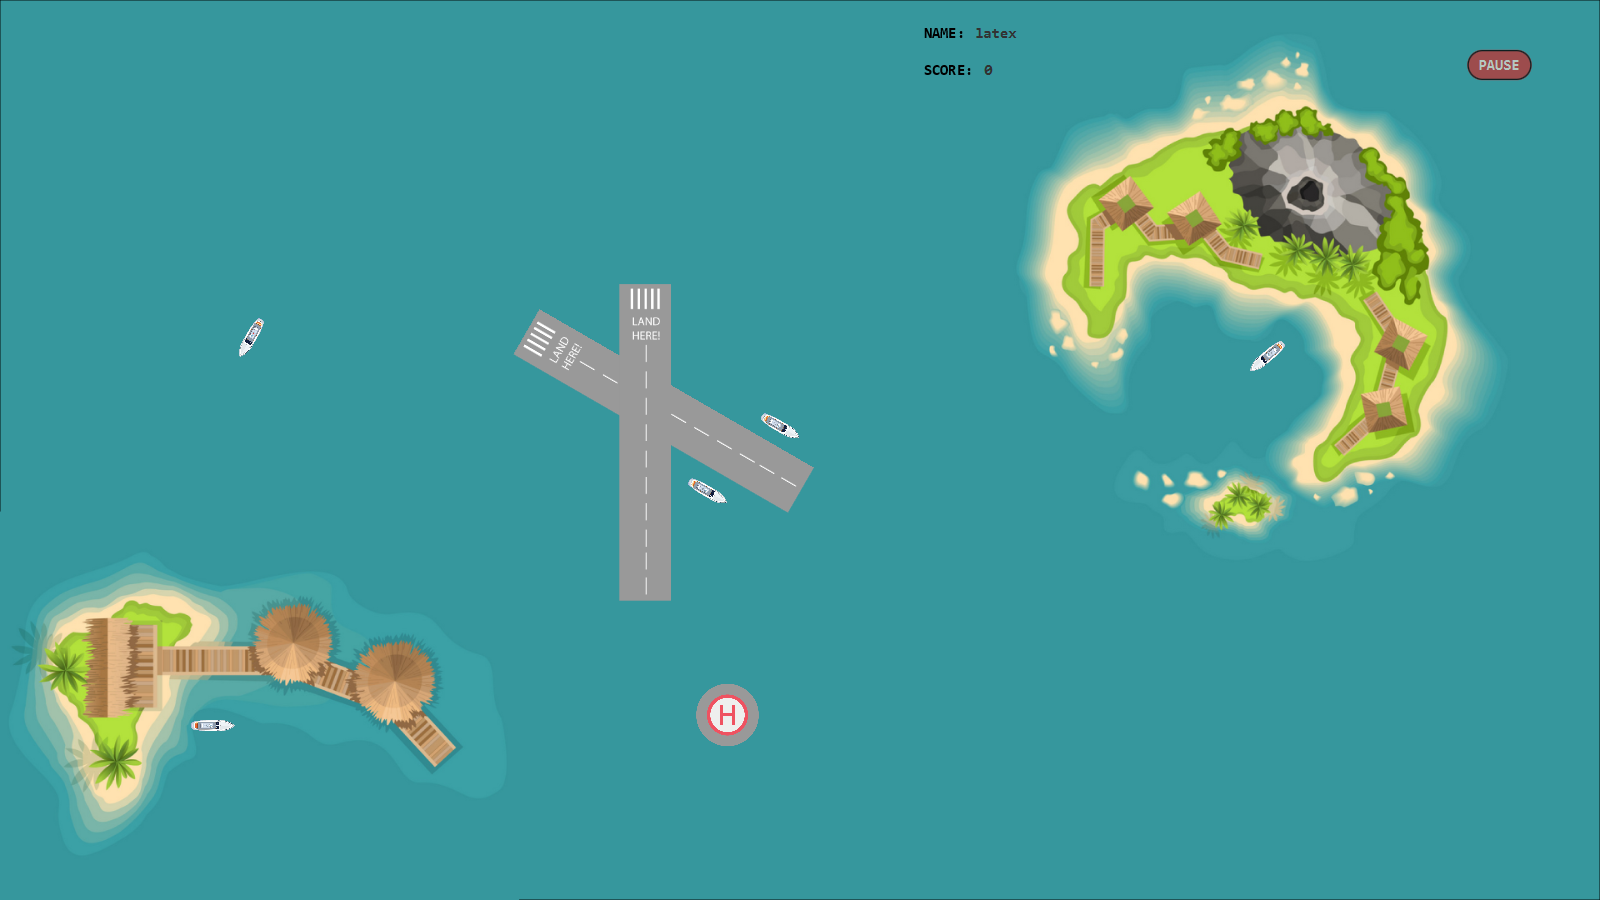
\includegraphics[width=\textwidth]{img/GuidaUtente/Seaside.png}
    \end{center}
    \caption{Mappa di gioco}
    \label{img:seaside}
\end{figure}

\clearpage

\noindent Per quanto riguarda l'atterraggio degli aerei, selezionare un aereo, l'aereo selezionato si presenta in \underline{maniera evidenziata} (vedi \figurename{ \ref{img:airplane}}), e tracciare un percorso (linea blu). Le piste di atterraggio sono 2, una per pista e sono demarcate con la scritta \qq{\texttt{LAND HERE}}. Sarà compito dell'utente evitare la collisione fra gli aerei e con i bordi della mappa (in entrambi i casi viene generata un'esplosione).
\begin{figure}[H]
    \begin{center}
        \centering
        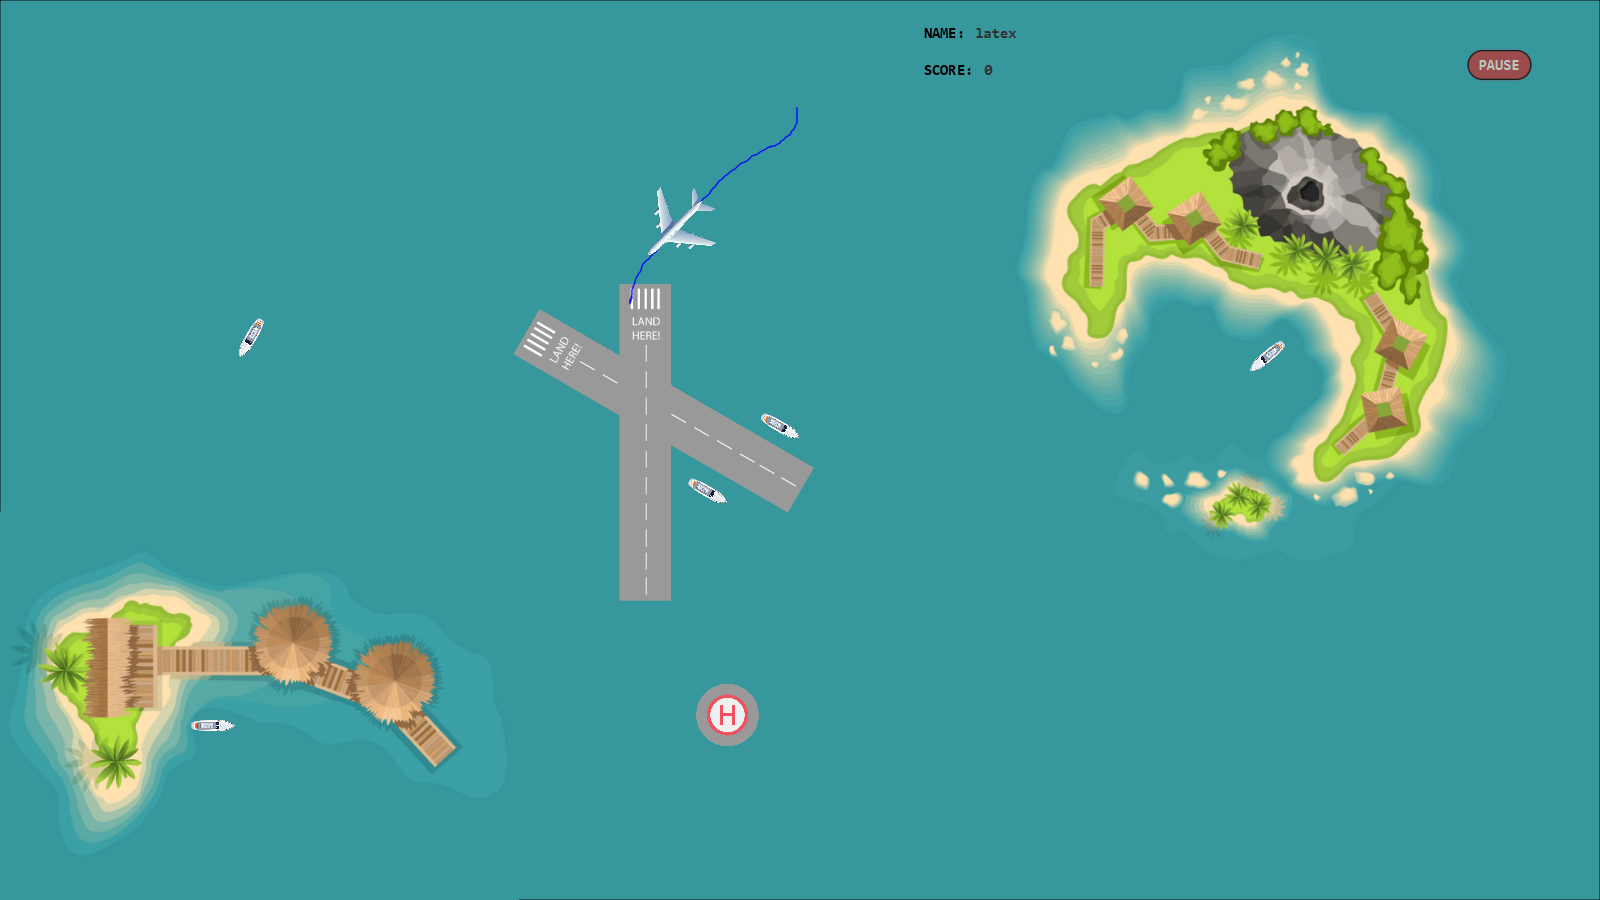
\includegraphics[width=\textwidth]{img/GuidaUtente/Landing.png}
    \end{center}
    \caption{Atterraggio aereo}
    \label{img:landing}
\end{figure}

\begin{figure}[H]
    \begin{center}
        \centering
        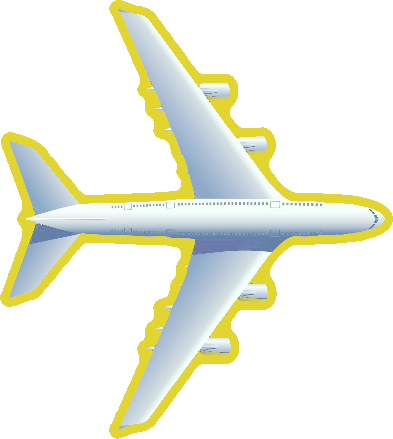
\includegraphics[scale = 0.3]{img/GuidaUtente/AirplaneSelected.png}
    \end{center}
    \caption{Aereo selezionato}
    \label{img:airplane}
\end{figure}
\end{document}
